\documentclass{article}

\usepackage{inputenc}[utf8]
\usepackage[T1]{fontenc}
\usepackage[a4paper]{geometry}
\usepackage{fancyhdr}
\usepackage{url}
\usepackage{hyperref}
\usepackage[ngerman]{babel}
\usepackage{graphicx}
\usepackage{pgfplots}
\usepackage{amsmath}
\usepackage{amssymb}
\usepackage{amsthm}

\usepackage{pdflscape}
\usepackage{caption}
\usepackage{subcaption}

% Generate external pdf and import
\pgfplotsset{width=9cm,compat=1.9}

\title{{\Huge Aufgabenblatt 04}\\Einführung in die Kryptographie PS}
\author{Andreas Schlager}


\begin{document}
    \pagestyle{fancy}
    \fancyhead{}
    \fancyhead[L]{Aufgabenblatt 04}
    \fancyhead[R]{Einführung in die Kryptographie}
    \fancyfoot{}
    \fancyfoot[L]{Andreas Schlager}
    \fancyfoot[R]{\thepage}
    \maketitle
    \tableofcontents
    \newpage

    \section{Aufgabe 14}
\textit{Erklären sie das Fuzzy Vault Scheme zur Erzeugung von kryptographischen Schlüsseln
aus biometrischen Messungen. Wann muss dieses Verfahren verwendet werden anstelle
des Fuzzy Commitment Schemes?}\vspace*{1em}\newline
Das Fuzzy Vault Scheme ist ein kryptographisches Verfahren, um Schlüssel mit unscharfen biometrischen Daten 
zu schützen. Im Gegensatz zu klassischer Verschlüsselung, die exakte Eingaben erfordert, 
erlaubt dieses Schema kleine Abweichungen, z.B wenn ein Fingerabdruck-Sensor bei jedem Scan leicht 
unterschiedliche Merkmale erfasst. Das Verfahren ist wie das Fuzzy Commitment Scheme (FCS) in zwei Stufen unterteilt,
der Registrierungs (Enrollment) und der Verifikation. Wie beim Fuzzy Commitment Scheme (FCS) wird während der Registrierung 
ein geheimer Schlüssel generiert und anschließend mit einem fehlerkorrigierenden Code (z. B. Reed-Solomon oder BCH-Code) 
kodiert, um Toleranz gegenüber leichten Abweichungen in den biometrischen Daten zu ermöglichen. Der Code wird als
Polynom kodiert. Beispielsweise würde der Code $7283$ zu einem Polynom mit Grad $3$ werden:
\[
    7283 \longrightarrow p(x)=7x^3 + 2x^2 + 8x^1 + 3
\]
Die biometrischen Merkmale (z.B. Minutien bei Fingerabdrücke) werden als eine Menge $\{x_1,x_2,\dots\}$ von Messpunkten erfasst. Da es
sich um eine Menge handelt, ist die Reihenfolge in der die Daten erfasst werden egal.
Jeder Messpunkt wird nun in das geheime Polynom eingesetzt, um Messpunkt-Ergebnis-Paare zu erhalten.
\[
    \{(x_1, p(x_1)),\ (x_2, p(x_2)),\ \dots\}
\]
Jedes Paar beschreibt einen Punkt auf der Kurve des Polynoms. Zuletzt werden die Punkte um "`falsche"' Punkte (Chaff-Points)
ergänzt. Dadurch kann ein Angreifer das Polynom nicht rekonstruieren, da ihm nicht bekannt ist, welche Punkte 
echte Messpunkte waren. Die Kombination aus den Polynompunkten und den Chaff-Points (auch \textit{Vault} $V$ genannt) wird
gespeichert.
\[
    V = \{(x_1, p(x_1)),\ (x_2, p(x_2)),\ \dots\}\cup \text{Chaff-Points}
\]
Bei der Verifikation werden wieder biometrische Messpunkte erfasst. Diese werden mit $V$ verglichen,
um die Chaff-Points herauszufiltern. Sofern die Daten nah genug an den ursprünglichen sind, kann 
das Polynom rekonstruiert werden. Aus dem Polynom leitet sich dann der Schlüssel ab.
\subsection{FCS vs. FVS}
Da das Fuzzy Vault Scheme mit Messpunkt-Mengen arbeitet, ist die Reihenfolge in der die Punkte gemessen werden
egal. Außerdem ist das FVS unempfindlich gegen das Hinzufügen oder Löschen von Datenpunkten (hohe Rauschtoleranz). 
Daher eignet es sich gut für die Verifikation über Fingermerkmale oder Gesichtserkennung. Chaff-Points bieten außerdem einen starken Schutz gegen
Brute-Force-Angriffe. FVS wird also vorallem dann eingesetzt, wenn ein hohes Sicherheitsmaß notwendig ist. 
Das Fuzzy Commitment Scheme ist besonders geeignet, wenn die Messdaten als Bitstring vorliegen, wie es bei Iris-Codes 
oder binär extrahierten Fingerabdruck-Merkmalen der Fall ist. Das FCS ist außerdem simpler und effizient,
wenn einfache fehlerkorrigierende Codes ausreichen.\newpage
    \section{Aufgabe 15}
\textit{Implementieren sie als einfaches Bildverschlüsselungsverfahren eine Permutation der
Zeilen eines Bildes. Dazu soll als Parameter (z.B. 1, 2, 4, ...) eine Anzahl von
horizontalen Bildblöcken definiert werden können, innerhalb derer jeweils die Permutationen angewendet werden (also Permutationen auf das ganze Bild für 1, Permutationen innhalb der oberen und unteren Bildhälfte für 2, u.s.w.). Versuchen
sie anschliessend, unter Ausnutzung der Tatsache dass ähnliche Bildzeilen meist
nebeneinander liegen, eine Ciphertext only Attacke gegen das verschlüsselte Bild
(für verschiedene Parameterwerte und Bilder).}\vspace*{1em}\newline
Die Implementierung der Ver- und Entschlüsselung wurde vollständig in der Programmiersprache
\textbf{Rust} geschrieben. Zur Bildmanipulation wird das \href{https://docs.rs/image/latest/image/}{image} Crate verwendet. 
\subsection{Verschlüsselungsverfahren}
Um ein Bild zu verschlüsseln, wird es aus dem Speicher geladen und durch \verb|permutation_cipher| mit der
gewünschten Blockanzahl verschlüsselt. Für
dieses Experiment werden $1,2,4,8,16,32$ Blöcke mit unterschiedlichen Bildern getestet. 
\begin{verbatim}
let original = image::open(&path).expect("Failed to open image");

for blocks in [1, 2, 4, 8, 16, 32] {
    let cipher_image = permutation_cipher(&original, blocks);
    cipher_image
        .save(format!("./img/out/{:02}_{}", blocks, filename))
        .expect("Failed to save image");
}
\end{verbatim}
Normalerweiße würde man das Verschlüsselungsverfahren deterministisch anhand eines
Schlüssel durchführen. Für den Zweck dieses Experiments soll allerdings 
kein Schlüssel ermittelt werden, also können die Zeilen innerhalb eines Blocks
einfach gemischt werden. Zwei Zeilen eines Blocks werden zufällig ausgewählt und
getauscht. Dieser Vorgang wird dann $1000$ Mal wiederholt, 
um einen gut gemischten Block zu erhalten.
\begin{verbatim}
fn permutation_cipher(original: &image::DynamicImage, blocks: u32) 
    let mut img = original.to_rgba8();
    let rows_per_block = img.height() / blocks;

    for block in 0..blocks {
        for _ in 0..1000 {
            let row1 = rng().random_range(0..rows_per_block) + 
                block * rows_per_block;
            let row2 = rng().random_range(0..rows_per_block) + 
                block * rows_per_block;

            swap_rows(&mut img, row1, row2);
        }
    }

    image::DynamicImage::ImageRgba8(img)
}
\end{verbatim}
\begin{figure}[h]
    \centering
    \begin{subfigure}[b]{0.3\textwidth}
        \centering
        
\includegraphics[width=\textwidth]{./img/tloztotk.png}
        \caption{Original}
    \end{subfigure}
    \hfill
    \begin{subfigure}[b]{0.3\textwidth}
        \centering
        
\includegraphics[width=\textwidth]{./img/cipher/04_tloztotk.png}
        \caption{4 Blöcke}
    \end{subfigure}
    \hfill
    \begin{subfigure}[b]{0.3\textwidth}
        \centering
        
\includegraphics[width=\textwidth]{./img/cipher/16_tloztotk.png}
        \caption{16 Blöcke}
    \end{subfigure}
    \caption{Verschlüsselung des Titelbilds von The Legend Of Zelda: Tears of the Kingdom}
    \label{fig:permutation_encryption_demo}
\end{figure}
Ist die Blockanzahl gering, gibt es mehr Anordnungen der Zeilen pro Block, wodurch das Bild
undeutlicher wird (siehe Abbildung \ref{fig:permutation_encryption_demo}). Bei einer
hohen Blockanzahl wird das Bild deutlicher, da es weniger mögliche Anordnungen innerhalb eines Blocks gibt.
\subsection{Ciphtext-only Attacke}
Da ähnliche Bildzeilen oft übereinander liegen, können die sie anhand ihrer Ähnlichkeit sortiert werden. Eine Möglichkeit ist
die Zeilen Pixel für Pixel zu vergleichen und jeweils die Distanz der Farben zu berechnen. In diesem Fall sind die Pixel
im RGBA Farbraum, das bedeutet vier Bytes pro Farbkanal (Rot, Grün, Blau und Alpha). Betrachtet man die Farbkanäle als Achsen und die
Farben als Punkte in einem mehrdimensionalen Raum, kann zwischen zwei Farben einfach die euklidische Distanz berechnet werden.
\begin{figure}[h]
    \centering
    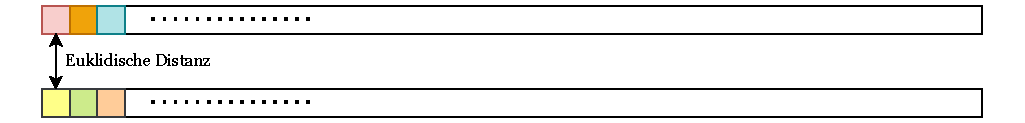
\includegraphics[width=\textwidth]{img/row_comparison.pdf}
    \caption{Zwei Bildzeilen, deren Pixel mittels euklidischer Distanz verglichen werden.}
\end{figure}
Seien $R,G,B,A\in\left[0;255\right]$ die Werte der jeweiligen Kanäle eines Pixels und $d$ die Distanz der Pixel.
\[
    d = \sqrt{(R_1 - R_2)^2 + (G_1 - G_2)^2 + (B_1 - B_2)^2 + (A_1 - A_2)^2}
\]
Die euklidische Distanz entspricht nicht umbedingt der menschlichen Wahrnehmung der Distanz zweier Farben, eignet sich allerdings
für die Sortierung der Bildzeilen. Unter den Zeilen des verschlüsselten Bilds, ist es schwierig die oberste Zeile zu identifizieren. Deshalb 
wird zur Vereinfachung angenommen, dass die oberste Zeile bereits an der richtigen Position ist. In der Realität ist das selten der Fall.
Dennoch können die Ergebnisse trotzdem erkennbar entschlüsselt werden (siehe \ref{sec:results_a15}). Von der obersten Zeile aus wird dann 
diejenige mit dem geringsten Unterschied zu den übrigen Zeilen identifiziert und mit der darauffolgenden Zeile getauscht (nearest-neighbour).

Zu Beginn werden die Zeilen des Bilds in ein Array (Vector) extrahiert, um sie später leichter zu vertauschen.
\begin{verbatim}
fn decipher(img: &RgbaImage) -> RgbaImage {
    let mut rows = img.rows()
        .map(|pixels| pixels.collect::<_>())
        .collect::<Vec<_>>();
    // ...
}
\end{verbatim}
Danach werden die Zeilen beginnend mit der obersten iteriert und der Index der besten Folgezeile bestimmt. 
Das beste Ergebnis wird dann an die nachfolgende Stelle verschoben. In diesem Fall reicht es aus, nur bis zur vorletzten Zeile
zu iterieren, da die letzte dann zwangsläufig schon die richtige Position haben muss.
\begin{verbatim}
for i in 0..img.height() as usize - 1 {
    if let Some(best_match) = nearest_neighbour(i, &rows) {
        rows.swap(i + 1, best_match);
    }
}
\end{verbatim}
Die sortierten Zeilen müssen nun nur noch zu einem neuen Bild zusammengefügt werden. Dafür wird die \verb|from_fn| Funktion der image Bibliothek verwendet,
die einfach jeden Pixel Stelle für Stelle übernimmt.
\begin{verbatim}
RgbaImage::from_fn(img.width(), img.height(), |x, y| {
    *rows[y as usize][x as usize]
})
\end{verbatim}
Die \verb|nearest_neighbour| Funktion berechnet den Index der Zeile mit der kleinsten Distanz zur Startzeile.
\begin{verbatim}
fn nearest_neighbour(start: usize, rows: &[Vec<&Rgba<u8>>]) -> Option<usize> {
    let (result, _) = (start + 1..rows.len())
        .map(|r| (r, similarity(&rows[r], &rows[start])))
        .min_by(|(_, a), (_, b)| a.partial_cmp(b).unwrap())?;
    Some(result)
}
\end{verbatim}
Die Ähnlichkeit zwischen zwei Zeilen wird anhand der euklidischen Distanz der Pixelfarben berechnet. 
Ein hoher Wert deutet auf geringe Ähnlichkeit hin, ein niedriger Wert auf hohe Ähnlichkeit.
\begin{verbatim}
fn similarity(r1: &[&Rgba<u8>], r2: &[&Rgba<u8>]) -> f32 {
    r1.iter()
        .zip(r2.iter())
        .map(|(&a, &b)| color::euclidean_distance(a.channels(), b.channels()))
        .sum()
}
\end{verbatim}
\newpage
\begin{landscape}
    \fancyhead{}
    \fancyfoot{}
    \newgeometry{left=1cm, right=-6cm, top=2.5cm, bottom=1cm}
    \renewcommand{\headrulewidth}{0pt}
\subsection{Ergebnisse}\label{sec:results_a15}
\begin{table}[h!]
    \begin{tabular}{|c|c|c|c|c|c|}
    \hline
    \textbf{Original} & \textbf{1 Block} & \textbf{4 Blöcke} & \textbf{8 Blöcke} & \textbf{16 Blöcke} & \textbf{32 Blöcke} \\
    \hline
    
\includegraphics[width=0.16\textwidth]{./img/tloztotk.png}& 
    
\includegraphics[width=0.16\textwidth]{./img/cipher/01_tloztotk.png}& 
    
\includegraphics[width=0.16\textwidth]{./img/cipher/04_tloztotk.png}& 
    
\includegraphics[width=0.16\textwidth]{./img/cipher/08_tloztotk.png}& 
    
\includegraphics[width=0.16\textwidth]{./img/cipher/16_tloztotk.png}& 
    
\includegraphics[width=0.16\textwidth]{./img/cipher/32_tloztotk.png}\\
    \hline
    &\textbf{Entschlüsselt 1} & \textbf{Entschlüsselt 4} & \textbf{Entschlüsselt 8} & \textbf{Entschlüsselt 16} & \textbf{Entschlüsselt 32} \\
    \hline
    &
    
\includegraphics[width=0.16\textwidth]{./img/decipher/01_tloztotk.png}& 
    
\includegraphics[width=0.16\textwidth]{./img/decipher/04_tloztotk.png}& 
    
\includegraphics[width=0.16\textwidth]{./img/decipher/08_tloztotk.png}& 
    
\includegraphics[width=0.16\textwidth]{./img/decipher/16_tloztotk.png}& 
    
\includegraphics[width=0.16\textwidth]{./img/decipher/32_tloztotk.png}\\
    \hline
    \end{tabular}
    \caption{Originalbild Titelbild von The Legend Of Zelda: Tears of the Kingdom, verschlüsselte und entschlüsselte Versionen}
\end{table}
\begin{table}[h!]
    \begin{tabular}{|c|c|c|c|c|c|}
    \hline
    \textbf{Original} & \textbf{1 Block} & \textbf{4 Blöcke} & \textbf{8 Blöcke} & \textbf{16 Blöcke} & \textbf{32 Blöcke} \\
    \hline
    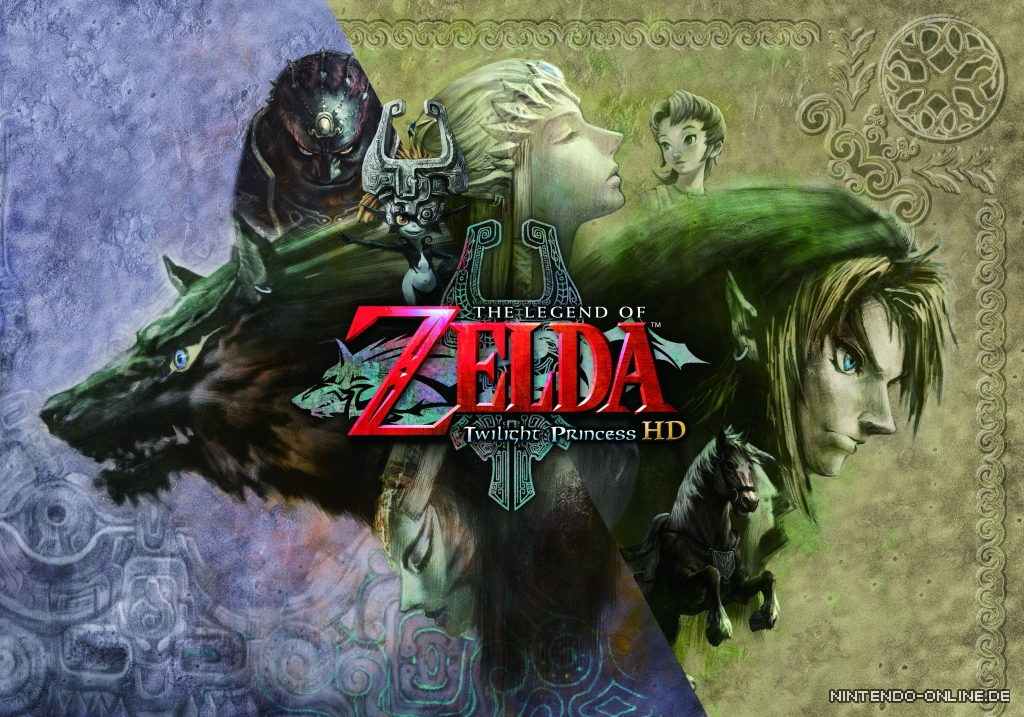
\includegraphics[width=0.16\textwidth]{./img/tloztp.png}& 
    
\includegraphics[width=0.16\textwidth]{./img/cipher/01_tloztp.png}& 
    
\includegraphics[width=0.16\textwidth]{./img/cipher/04_tloztp.png}& 
    
\includegraphics[width=0.16\textwidth]{./img/cipher/08_tloztp.png}& 
    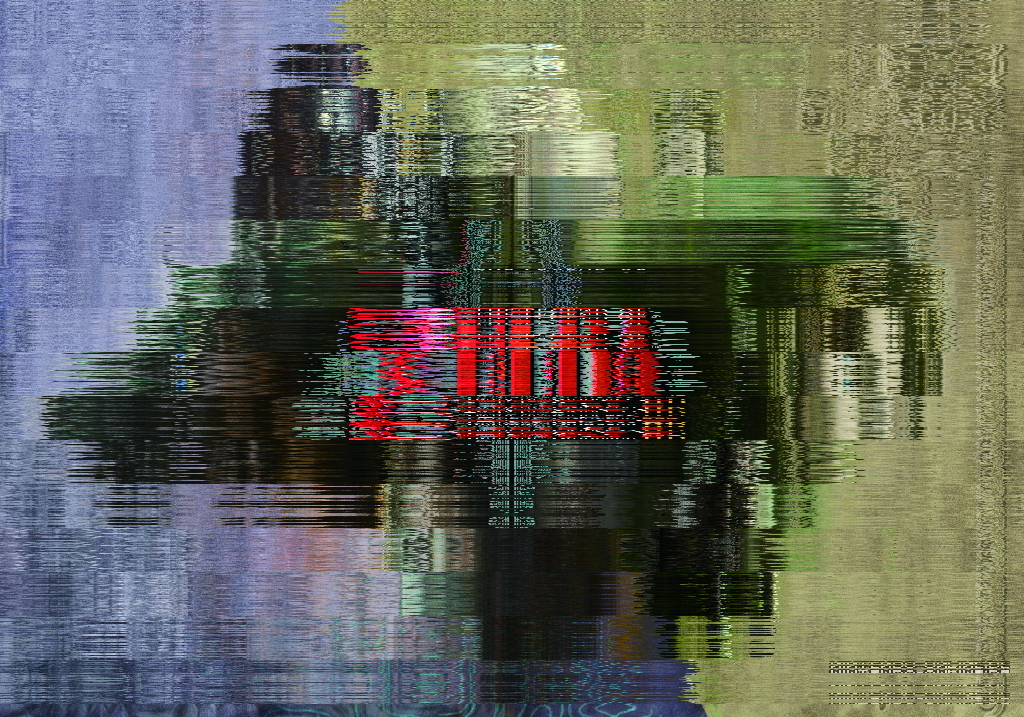
\includegraphics[width=0.16\textwidth]{./img/cipher/16_tloztp.png}& 
    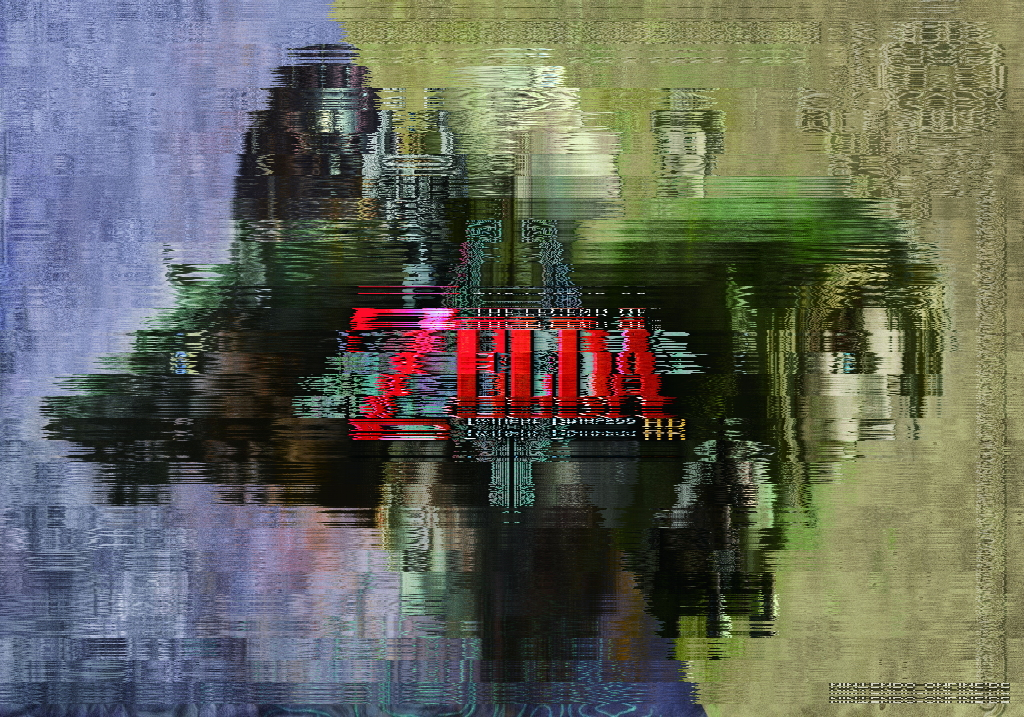
\includegraphics[width=0.16\textwidth]{./img/cipher/32_tloztp.png}\\
    \hline
    &\textbf{Entschlüsselt 1} & \textbf{Entschlüsselt 4} & \textbf{Entschlüsselt 8} & \textbf{Entschlüsselt 16} & \textbf{Entschlüsselt 32} \\
    \hline
    &
    
\includegraphics[width=0.16\textwidth]{./img/decipher/01_tloztp.png}& 
    
\includegraphics[width=0.16\textwidth]{./img/decipher/04_tloztp.png}& 
    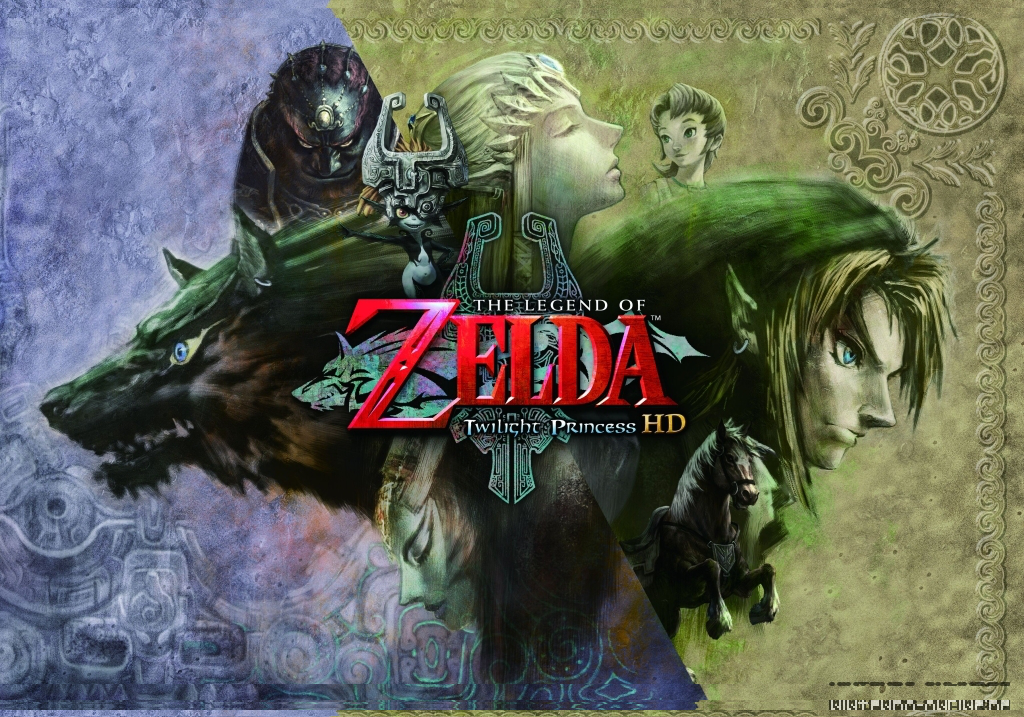
\includegraphics[width=0.16\textwidth]{./img/decipher/08_tloztp.png}& 
    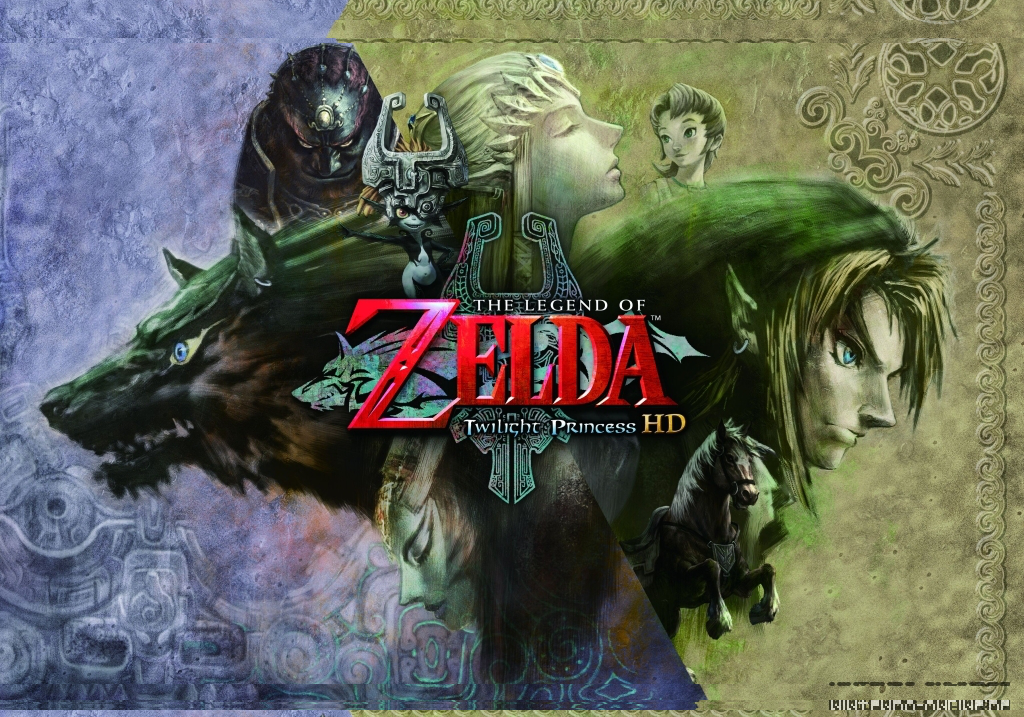
\includegraphics[width=0.16\textwidth]{./img/decipher/16_tloztp.png}& 
    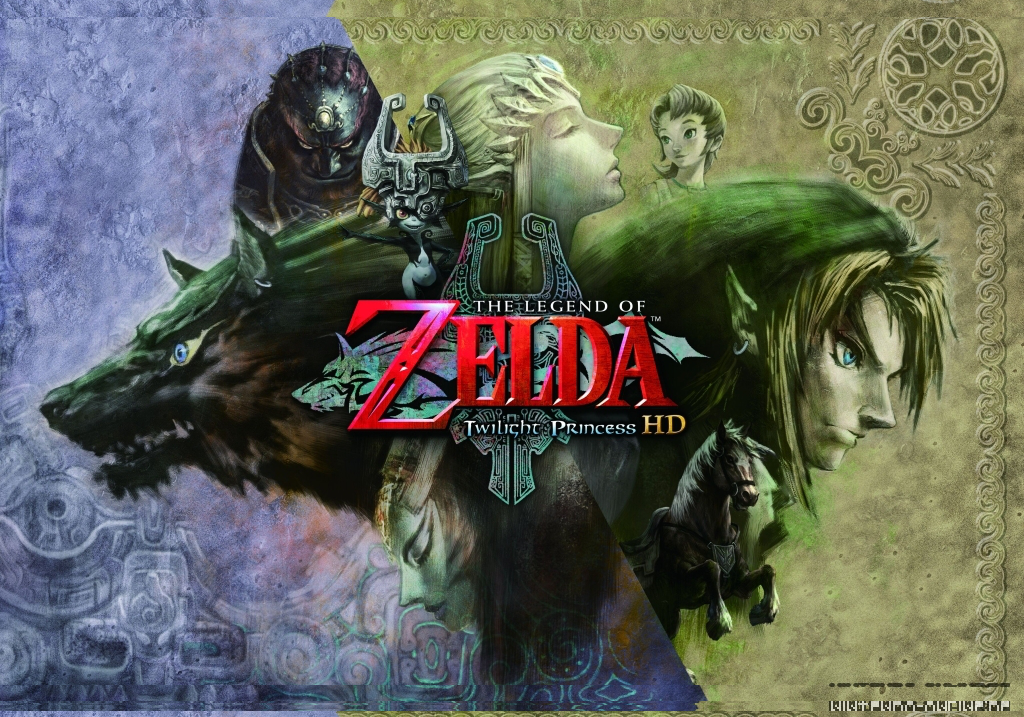
\includegraphics[width=0.16\textwidth]{./img/decipher/32_tloztp.png}\\
    \hline
    \end{tabular}
    \caption{Originalbild Titelbild von The Legend Of Zelda: Twilight Princess, verschlüsselte und entschlüsselte Versionen}
\end{table}
\newpage
\begin{table}[h!]
    \begin{tabular}{|c|c|c|c|c|c|}
    \hline
    \textbf{Original} & \textbf{1 Block} & \textbf{4 Blöcke} & \textbf{8 Blöcke} & \textbf{16 Blöcke} & \textbf{32 Blöcke} \\
    \hline
    
\includegraphics[width=0.16\textwidth]{./img/test.png}& 
    
\includegraphics[width=0.16\textwidth]{./img/cipher/01_test.png}& 
    
\includegraphics[width=0.16\textwidth]{./img/cipher/04_test.png}& 
    
\includegraphics[width=0.16\textwidth]{./img/cipher/08_test.png}& 
    
\includegraphics[width=0.16\textwidth]{./img/cipher/16_test.png}& 
    
\includegraphics[width=0.16\textwidth]{./img/cipher/32_test.png}\\
    \hline
    &\textbf{Entschlüsselt 1} & \textbf{Entschlüsselt 4} & \textbf{Entschlüsselt 8} & \textbf{Entschlüsselt 16} & \textbf{Entschlüsselt 32} \\
    \hline
    &
    
\includegraphics[width=0.16\textwidth]{./img/decipher/01_test.png}& 
    
\includegraphics[width=0.16\textwidth]{./img/decipher/04_test.png}& 
    
\includegraphics[width=0.16\textwidth]{./img/decipher/08_test.png}& 
    
\includegraphics[width=0.16\textwidth]{./img/decipher/16_test.png}& 
    
\includegraphics[width=0.16\textwidth]{./img/decipher/32_test.png}\\
    \hline
    \end{tabular}
    \caption{Zwei Farben Bild, mit schrägen Verlauf. Der Vergleich zweier Zeilen wird erleichtert.}
\end{table}
\begin{table}[h!]
    \begin{tabular}{|c|c|c|c|c|c|}
    \hline
    \textbf{Original} & \textbf{1 Block} & \textbf{4 Blöcke} & \textbf{8 Blöcke} & \textbf{16 Blöcke} & \textbf{32 Blöcke} \\
    \hline
    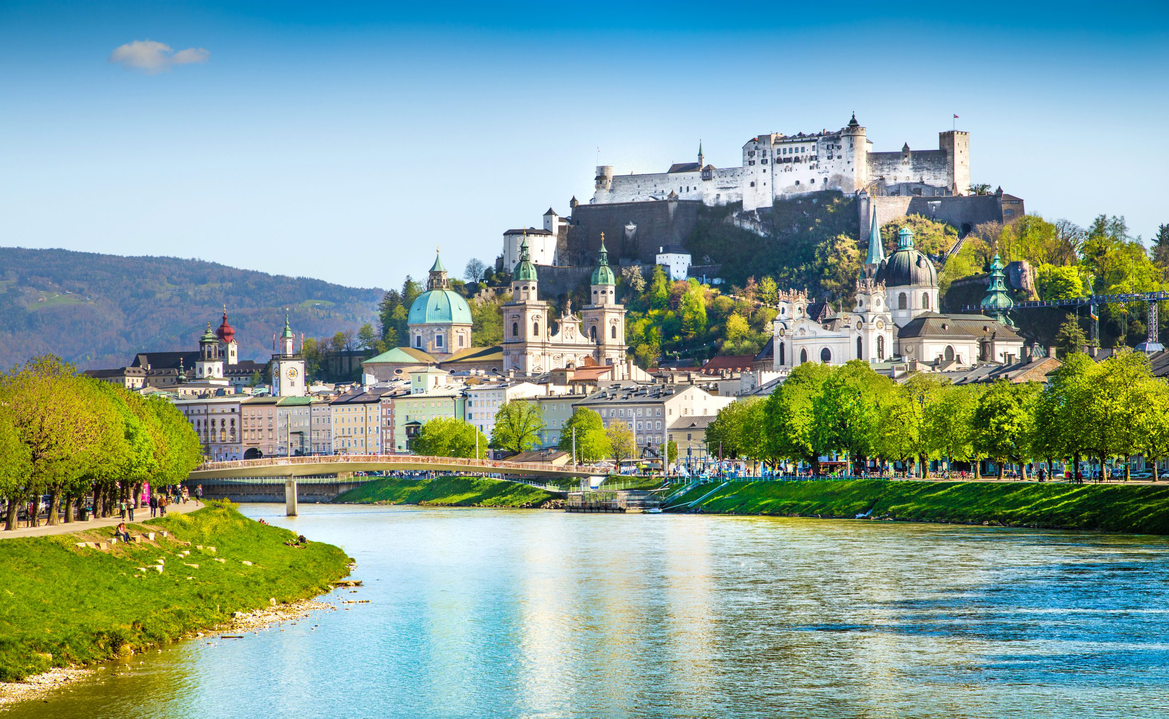
\includegraphics[width=0.16\textwidth]{./img/salzburg.png}& 
    
\includegraphics[width=0.16\textwidth]{./img/cipher/01_salzburg.png}& 
    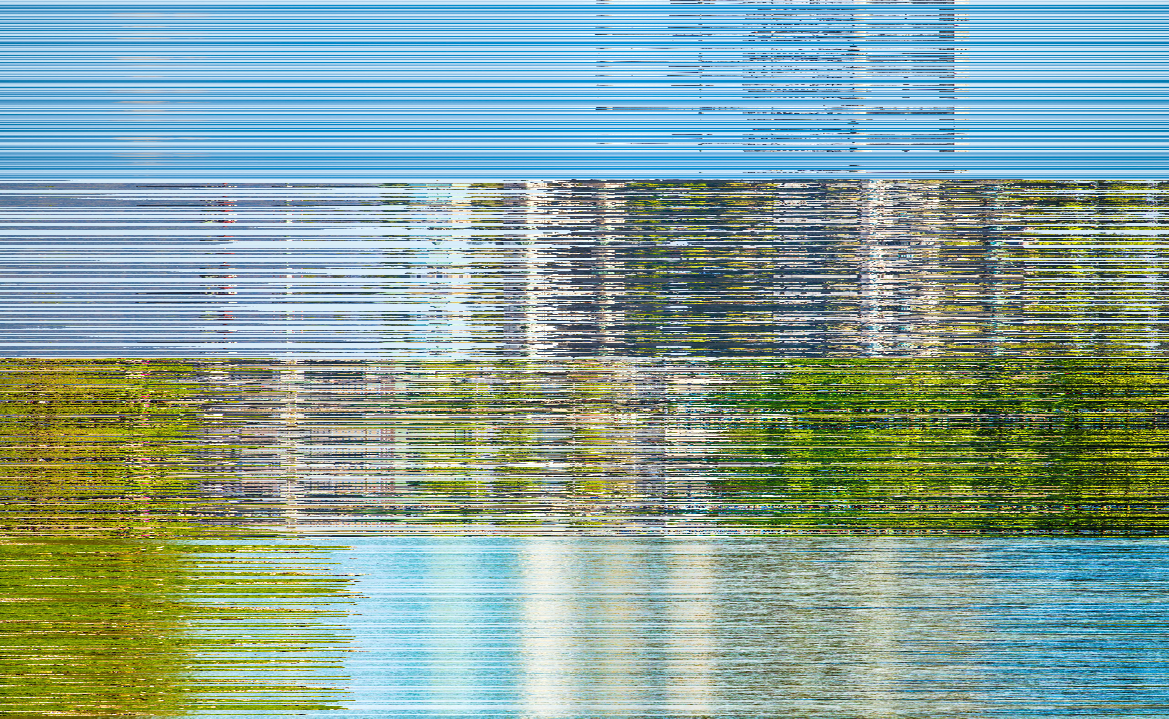
\includegraphics[width=0.16\textwidth]{./img/cipher/04_salzburg.png}& 
    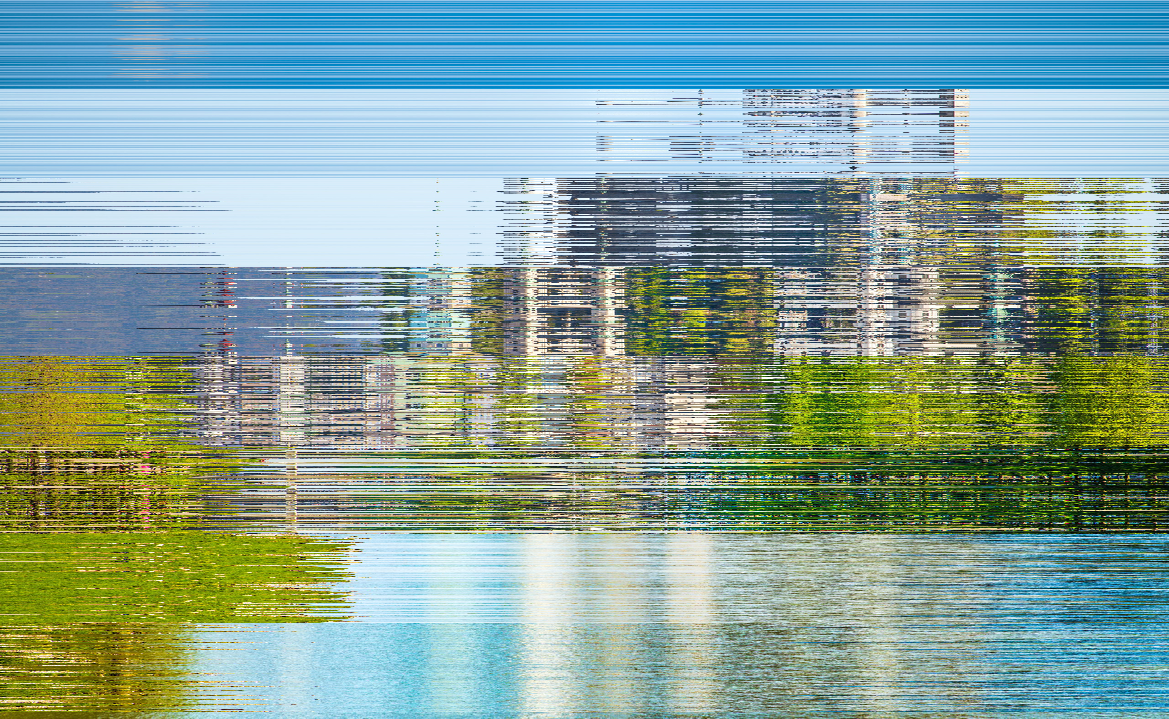
\includegraphics[width=0.16\textwidth]{./img/cipher/08_salzburg.png}& 
    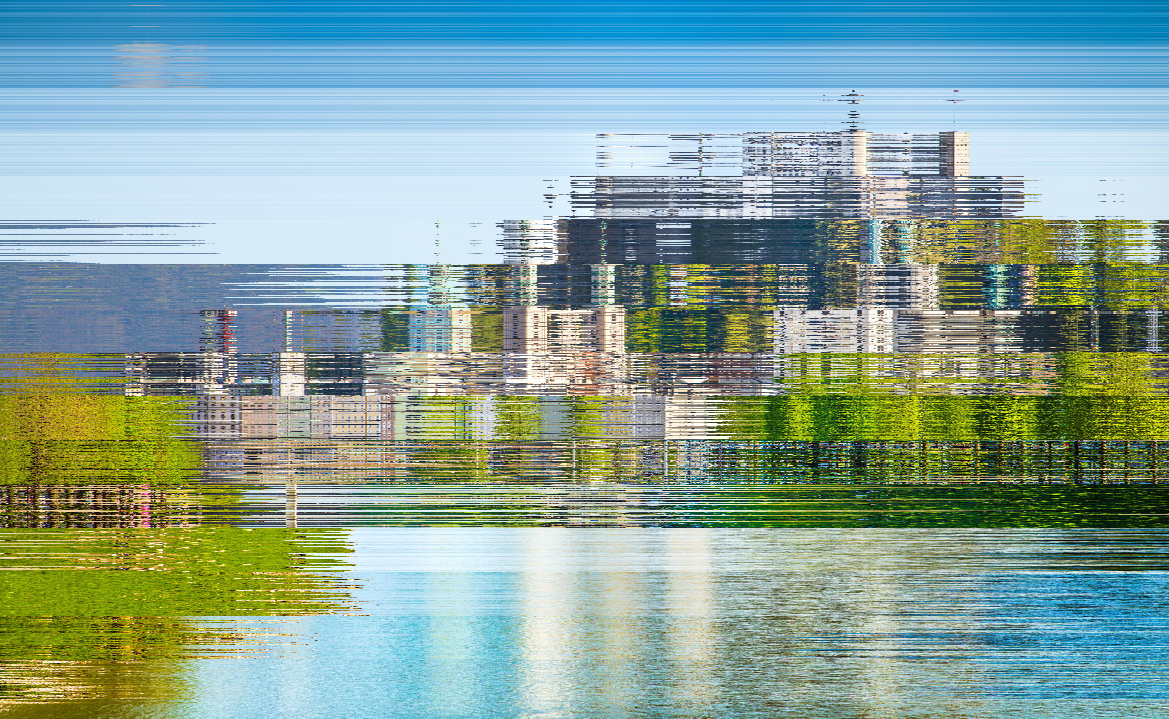
\includegraphics[width=0.16\textwidth]{./img/cipher/16_salzburg.png}& 
    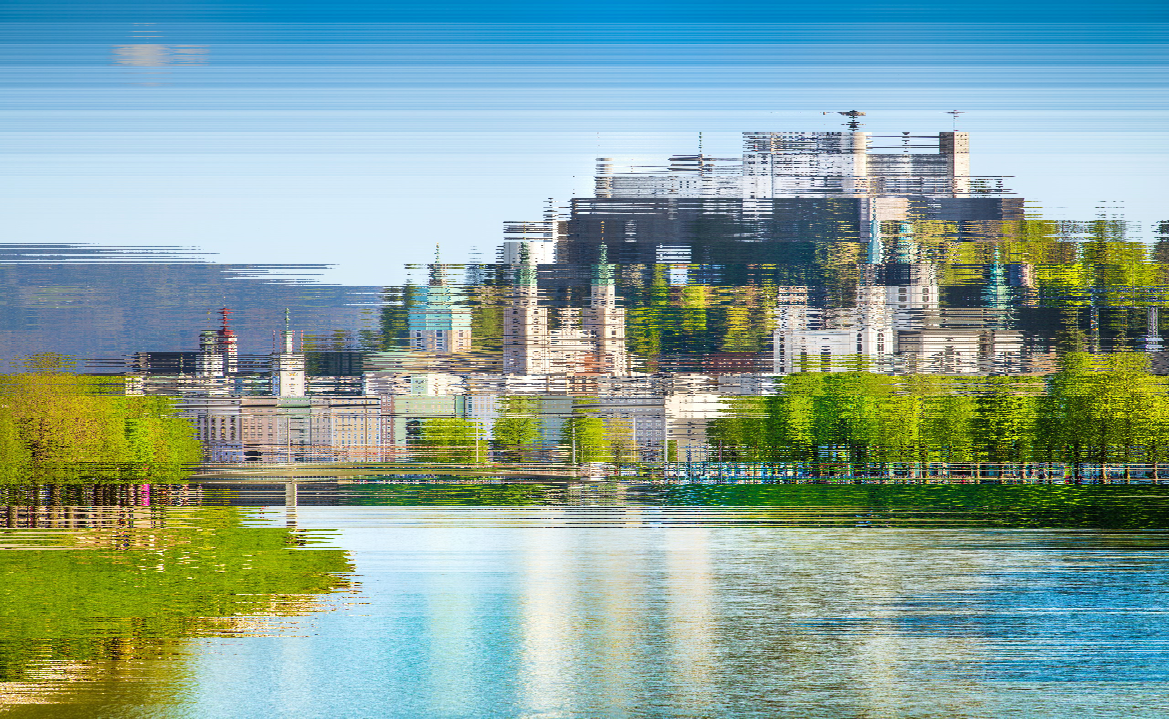
\includegraphics[width=0.16\textwidth]{./img/cipher/32_salzburg.png}\\
    \hline
    &\textbf{Entschlüsselt 1} & \textbf{Entschlüsselt 4} & \textbf{Entschlüsselt 8} & \textbf{Entschlüsselt 16} & \textbf{Entschlüsselt 32} \\
    \hline
    &
    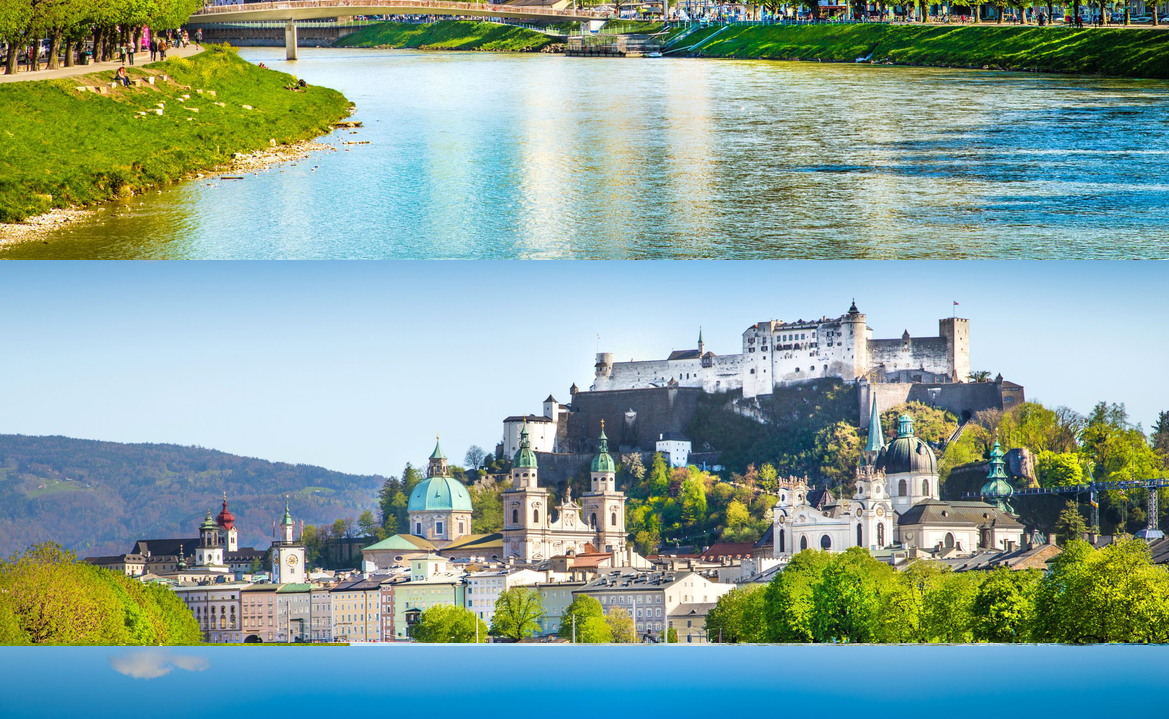
\includegraphics[width=0.16\textwidth]{./img/decipher/01_salzburg.png}& 
    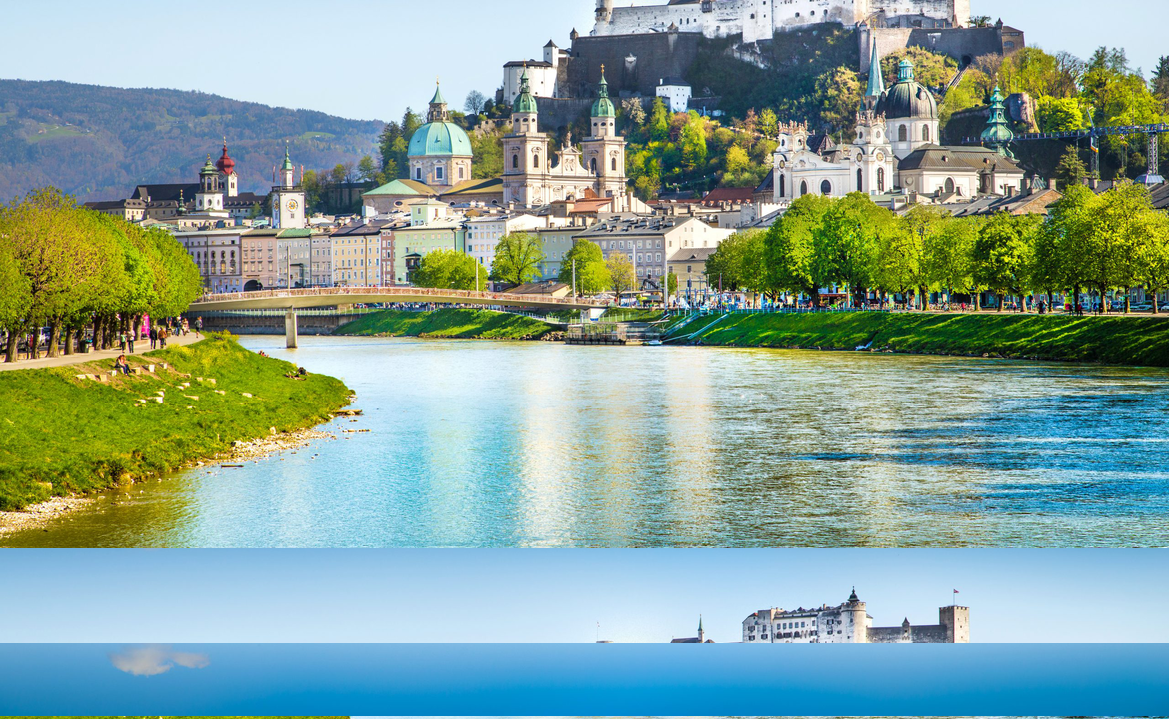
\includegraphics[width=0.16\textwidth]{./img/decipher/04_salzburg.png}& 
    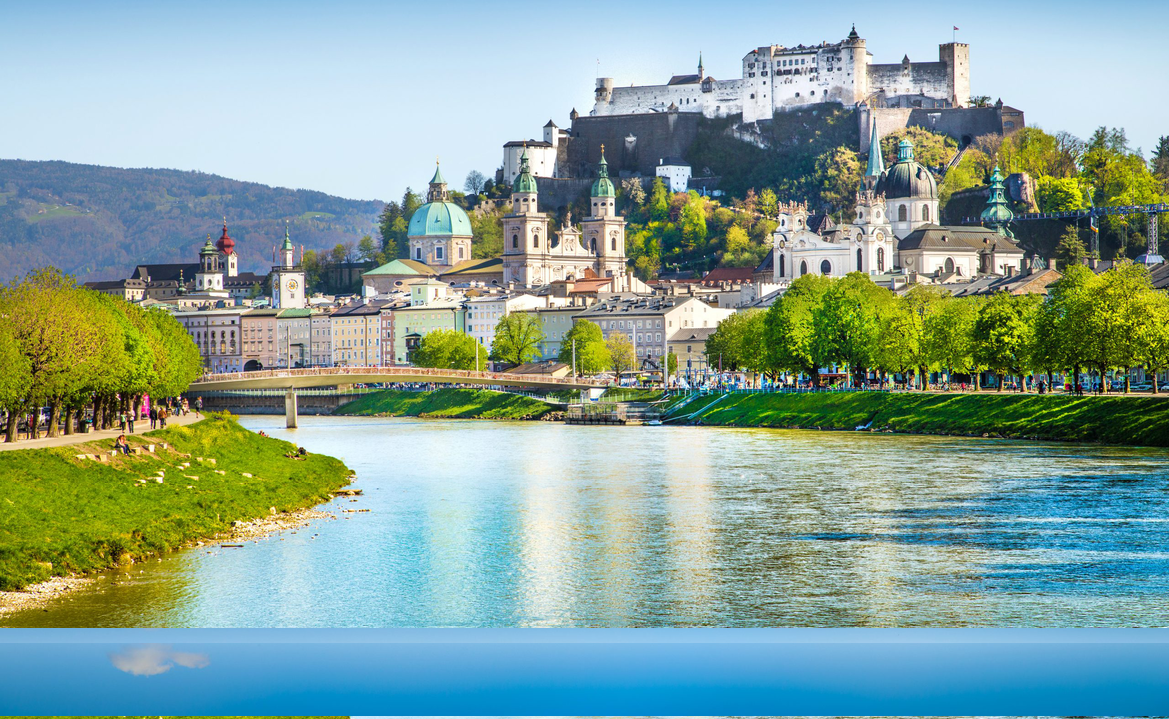
\includegraphics[width=0.16\textwidth]{./img/decipher/08_salzburg.png}& 
    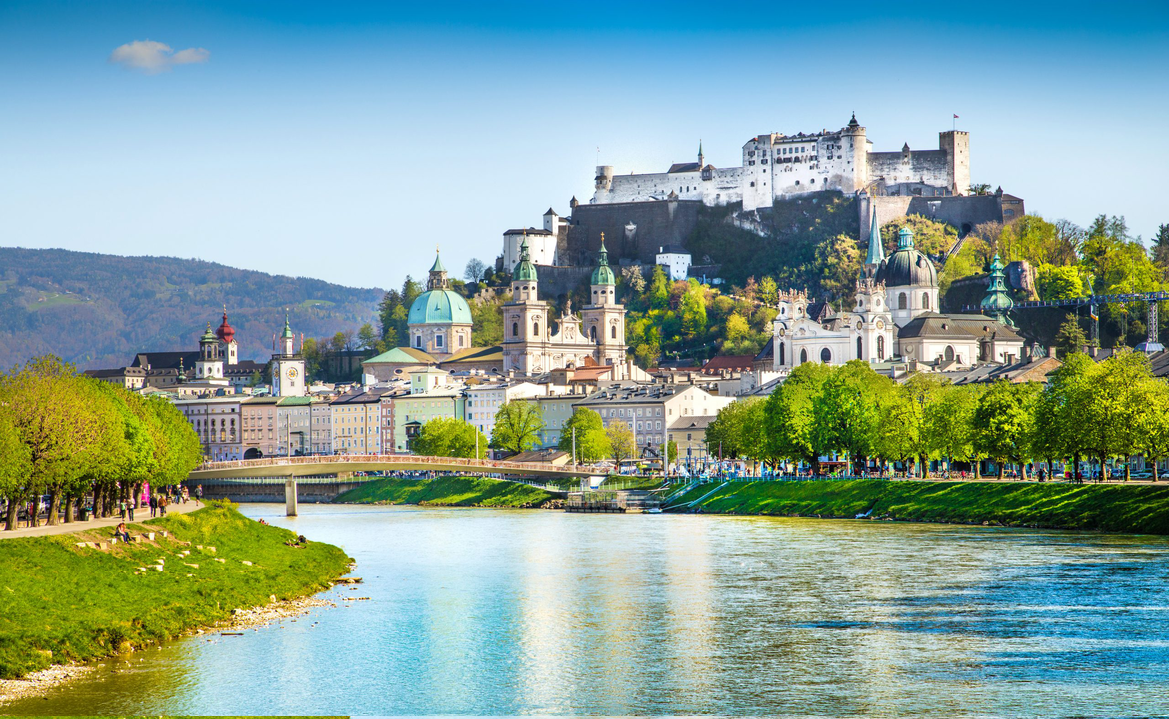
\includegraphics[width=0.16\textwidth]{./img/decipher/16_salzburg.png}& 
    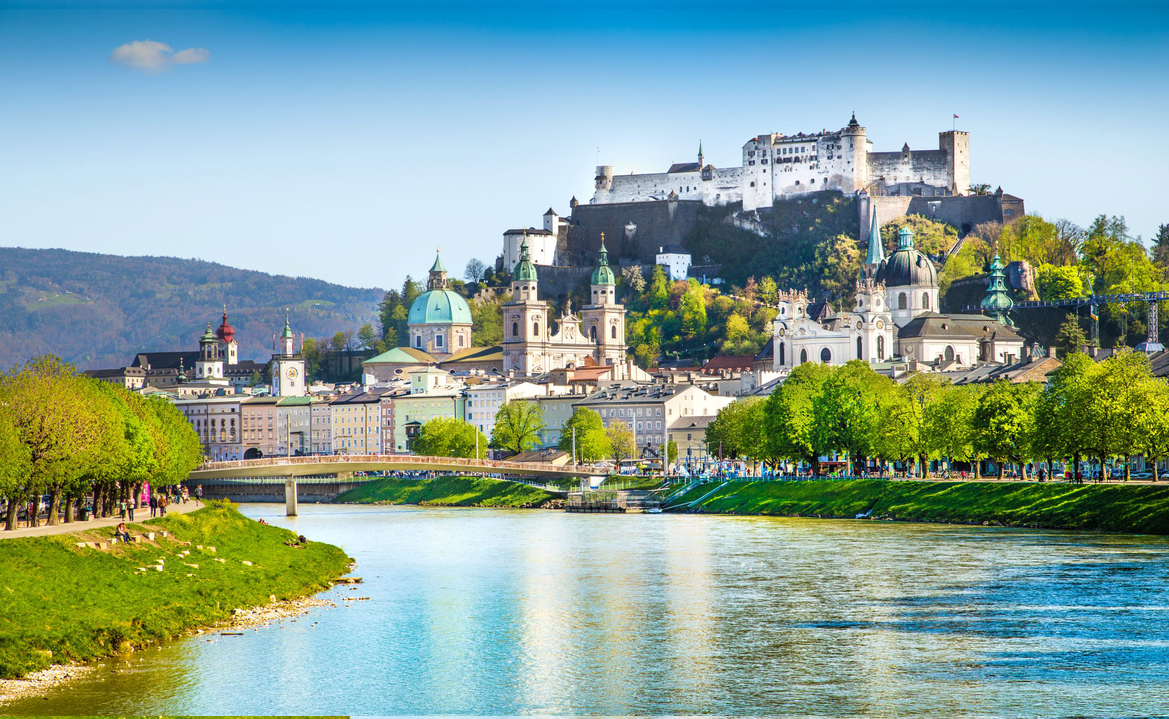
\includegraphics[width=0.16\textwidth]{./img/decipher/32_salzburg.png}\\
    \hline
    \end{tabular}
    \caption{Originalbild von Salzburg, verschlüsselte und entschlüsselte Versionen}
\end{table}
\end{landscape}
\newpage
\subsection{Fazit}
Die experimentellen Ergebnisse zeigten, dass die Blockanzahl einen entscheidenden Einfluss auf die 
Klarheit des verschlüsselten Bildes hat. Mit einer geringeren Blockanzahl wird das Bild stärker verzerrt, 
während eine höhere Blockanzahl zu einer weniger verschlüsselten Darstellung führt.
Die Ciphertext-only-Attacke, die auf der Ähnlichkeit benachbarter Bildzeilen basiert, 
konnte erfolgreich angewendet werden, wobei die Bilder Schnittstellen aufweisen oder manchmal auf dem Kopf stehen.
Die Schnittstellen sind auf die ursprüngliche Annahme, dass die erste Zeile bereits korrekt ist, zurückzuführen.
Nach der Permutation ist die oberste Zeile eine zufällige aus dem ersten Block. Je kleiner der Block ist,
desto höher ist die Wahrscheinlicht die tatsächlich richtige Zeile zu erwischen. Die darauffolgenden Zeilen
konnten richtig geordnet werden, bis eine Randzeile des Originalbilds erreicht und kein guter
Match mehr gefunden wurde. Dann wählt der Algorithmus mehr oder weniger eine zufällige der übrigen Zeilen
aus und arbeitet mit dieser weiter. Pro Zeile (exkl. Randzeilen) gibt es auch immer zwei Zeilen,
die gute Nachbarn wären. Zum einen ist das die Zeile im Originalbild, die darüber liegt und zum anderen
die darunter liegende. Je nach Wahl wird das Bild möglicherweise verkehrt herum aufgebaut.\newpage
    \section{Aufgabe 16}
\textit{Implementieren sie die in der VO besprochene short Key XOR Verschlüsselung (Text
wird über ASCII-Nummern binär dargestellt und mit ensprechendem “binärem” Text
Key XOR verschlüsselt, variable Key-länge für Experimente erforderlich). Bestimmen 
sie mit der in der VO besprochenen “Counting Coincidences” Methode die 
Länge des jeweils verwendeten Keys.}\vspace*{1em}\newline
Zuerst muss ein zufällig Schlüssel mit festlegbarer Länger erzeugt werden. Dafür wurde die
Funktion \verb|generate_key| erstellt, die eine gewünschte Schlüssellänge erhält und einen entsprechenden 
Key erzeugt.
\begin{verbatim}
fn generate_key(length: usize) -> Vec<u8> {
    rng().random_iter().take(length).collect::<Vec<u8>>()
}
\end{verbatim}
Der Plaintext kann dann über einen Aufruf der Funktion \verb|short_key_xor| zusammen mit dem Key
verschlüsselt werden. Falls die Länge des Plaintexts kein Vielfaches der Schlüssellänge ist, wird der String
mit dem Zeichen $X$ aufgepolstert. Die Füllzeichen werden während der Iteration über die Zeichen des Plaintexts
angehängt. Die Bytes des Schlüssel wiederholen sich, indem die Position des Zeichens im Plaintext modulo der Schlüssellänge
gerechnet wird. Für die Verschlüsselung selbst werden die Zeichen des Strings in ASCII umgewandelt und mit dem Key geXORt.
\begin{verbatim}
fn short_key_xor(text: &str, key: &[u8]) -> Vec<u8> {
    let padding = key.len() - text.len() % key.len();
    text.chars()
        .chain(std::iter::repeat_n('X', padding))
        .enumerate()
        .map(|(i, c)| c as u8 ^ key[i % key.len()])
        .collect()
}
\end{verbatim}
Um die Länge des Schlüssel zu bestimmen wird der Ciphertext mit jeder möglichen verschobenen Variante von sich selbst
verglichen. In jeder Iteration werden die übereinstimmenden Bytes, für den entsprechenden \verb|offset|, gezählt. 
Ist die relative Häufigkeit der gleichen Bytes $>6.65\%$, so ist \verb|offset| die Schlüssellänge. Wird keine
passende Verschiebung gefunden, wir angenommen, dass der Schlüssel gleich lang wie der originale Text war (Long-Key XOR).
\begin{verbatim}
fn counting_coincidences(text: &[u8]) -> usize {
    for offset in 1..text.len() {
        let same_bytes = text
            .iter()
            .zip(text.iter().chain(text).skip(offset))
            .filter(|&(a, b)| a == b)
            .count() as f32
            / text.len() as f32;
        if same_bytes > 0.06 {
            return offset;
        }
    }
    text.len()
}
\end{verbatim}
Da sich der IOC bei der korrekten Verschiebung $6.65\%$ annähert, wurde hier ein Schwellwert von $>6\%$ festgelegt. Dadurch
werden die korrekten Schlüssellänge auch bei kürzeren Texten identifiziert. Der Algorithmus stoppt sobald ein Wert gefunden wird,
der die Schwelle überschreitet.
\subsection{Ergebnisse}
\textbf{Plaintext}: \textit{Methode von Kasiski: Identische sich wiederholdende Teile des Plaintexts ge-XORed mit dem gleichen Teil des Keys ergeben sich
wiederholende identische Ciphertext Teile. Die Groesse des Shifts
zwischen dem Beginn solcher sich wiederholenden Teile im
Ciphertext sollte daher ein Vielfaches der Key-Laenge sein. Die
Analyse der gemeinsamen Faktoren dieser Shifts identifiziert den
haeufigsten Faktor der dann der Key-laenge entspricht.} (siehe Tabelle \ref{tab:CC_result_1})\vspace*{1em}\newline
Die verwendet Schlüssellänge steht über den Tabellenwerten, die korrekte Verschiebung ist fett markiert. Der letzte Tabelleneintrag
ist das Ergebnisse des Algorithmus, die geschätzte Schlüssellänge.
\begin{table}[h]
    \begin{subtable}[t]{0.3\textwidth}
        \centering
        \begin{tabular}{c|c}
            \multicolumn{2}{l}{\textbf{Keylength: 8}}\\\hline
            SHIFT & IOC\\\hline
            01&      1.14\%\\
            02&      0.45\%\\
            03&      0.45\%\\
            04&      0.00\%\\
            05&      0.45\%\\
            06&      0.00\%\\
            07&      0.23\%\\
            \textbf{08}&      7.95\%
        \end{tabular}
    \end{subtable}
    \begin{subtable}[h]{0.3\textwidth}
        \centering
        \begin{tabular}{c|c}
            \multicolumn{2}{l}{\textbf{Keylength: 13}}\\\hline
            SHIFT & IOC\\\hline
            01 &      0.00\%\\
            02 &      0.23\%\\
            03 &      0.00\%\\
            04 &      0.45\%\\
            05 &      0.23\%\\
            06 &      0.00\%\\
            07 &      0.23\%\\
            08 &      0.23\%\\
            09 &      0.00\%\\
            10 &      0.00\%\\
            11 &      0.68\%\\
            12 &      0.23\%\\
            \textbf{13} &      7.69\%
        \end{tabular}
    \end{subtable}
    \begin{subtable}[h]{0.3\textwidth}
        \centering
        \begin{tabular}{c|c}
            \multicolumn{2}{l}{\textbf{Keylength: 19}}\\\hline
            SHIFT & IOC\\\hline
            01&      0.46\%\\
            02&      0.00\%\\
            03&      0.23\%\\
            04&      0.69\%\\
            05&      0.23\%\\
            06&      0.23\%\\
            07&      0.23\%\\
            08&      0.23\%\\
            09&      0.00\%\\
            10&      0.23\%\\
            11&      0.46\%\\
            12&      0.00\%\\
            13&      0.23\%\\
            14&      0.46\%\\
            15&      0.23\%\\
            16&      0.00\%\\
            17&      0.23\%\\
            18&      0.00\%\\
            \textbf{19}&      6.64\%
        \end{tabular}
    \end{subtable}
    \caption{IOC Werte für unterschiedliche Keylängen, bei unterschiedliche Shifts}
    \label{tab:CC_result_1}
\end{table}\newline
Verwendet man einen kürzeren Plaintext, hat das Verfahren nicht bei jeder Schlüssellänge funktioniert.
Es sind nicht genug Werte vorhanden, um den IOC ausreichend an den Schwellwert anzunähern. Manchmal wurde
nur ein Vielfaches der Schlüssellänge erkannt, oder kein Wert hat den Schwellwert erreicht.\vspace*{1em}\newline
\textbf{Plaintext}: \textit{Wird nicht ein kurzer repetitiver Schluessel verwendet sondern einer der
die gleiche Laenge aufweist wie der Plaintext, spricht man von OTP
Verschluesselung"} (siehe Tabelle \ref{tab:CC_result_2})
\begin{table}[h]
    \begin{subtable}[t]{0.25\textwidth}
        \centering
        \begin{tabular}{c|c}
            \multicolumn{2}{l}{\textbf{Keylength: 8}}\\\hline
            SHIFT & IOC\\\hline
            01&      0.62\%\\
            02&      0.00\%\\
            03&      0.00\%\\
            04&      0.62\%\\
            05&      0.00\%\\
            06&      0.62\%\\
            07&      0.00\%\\
            \textbf{08}&      8.12\%
        \end{tabular}
        \caption{Schlüssellänge konnte richtig identifiziert werden.}
    \end{subtable}
    \hfill
    \begin{subtable}[h]{0.25\textwidth}
        \centering
        \begin{tabular}{c|c}
            \multicolumn{2}{l}{\textbf{Keylength: 12}}\\\hline
            SHIFT & IOC\\\hline
            01&      0.00\%\\
            02&      0.60\%\\
            03&      1.79\%\\
            04&      0.60\%\\
            05&      0.60\%\\
            06&      0.60\%\\
            07&      1.19\%\\
            08&      1.19\%\\
            09&      1.19\%\\
            10&      0.00\%\\
            11&      0.00\%\\
            \textbf{12}&      5.95\%\\
            13&      0.60\%\\
            14&      0.00\%\\
            15&      0.00\%\\
            16&      1.19\%\\
            17&      0.60\%\\
            18&      0.60\%\\
            19&      0.00\%\\
            20&      0.60\%\\
            21&      0.60\%\\
            22&      0.60\%\\
            23&      0.60\%\\
            24&      7.74\%
        \end{tabular}
        \subcaption{Schlüssellänge wurde als ein Vielfaches der richtigen Länge identifiziert.}
    \end{subtable}
    \hfill
    \begin{subtable}[h]{0.25\textwidth}
        \centering
        \begin{tabular}{c|c}
            \multicolumn{2}{l}{\textbf{Keylength: 19}}\\\hline
            SHIFT & IOC\\\hline
            01&      0.58\%\\
            02&      0.58\%\\
            03&      0.00\%\\
            04&      0.00\%\\
            05&      0.58\%\\
            06&      0.58\%\\
            07&      0.00\%\\
            08&      0.00\%\\
            09&      1.17\%\\
            10&      1.17\%\\
            11&      0.00\%\\
            12&      0.00\%\\
            13&      0.00\%\\
            14&      0.00\%\\
            15&      0.00\%\\
            16&      0.00\%\\
            17&      0.58\%\\
            18&      0.00\%\\
            \textbf{19}&      4.68\%\\
            20&      0.58\%\\
            $\vdots$ & $\vdots$\\
            168&     0.00\%\\
            169&     0.58\%\\
            170&     0.58\%
        \end{tabular}
        \subcaption{Schlüssellänge konnte nicht gefunden werden}
    \end{subtable}
    \caption{Zweites Experiment mit kürzerem Text. Nicht jede Schlüssellänge wird richtig erkannt.}
    \label{tab:CC_result_2}
\end{table}
\subsection{Fazit}
Sofern ausreichend Text vorhanden ist, bietet die Counting Coincidences Methode einen guten Weg um die Schlüssellänge
zu bestimmen. Falls der Text zu kurz ist, enstehen falsche Ergebnisse, die entweder ein Vielfaches der richtigen Länge sind,
oder den Schlüssel gleich lang wie den Text schätzen.\newpage
    \section{Zeitaufwand}
Zeiteinheiten sind in Stunden [h].
\begin{table}[h]
    \begin{tabular}{l|ccc|r}
        Aufgabe & Coding & Recherche & Schreiben & $\sum$\\\hline
        Aufgabe 14 & 0 & 0.5 & 1 & 1.5 \\
        Aufgabe 15 & 5 & 0.5 & 6 & 11.5 \\
        Aufgabe 16 & 1.5 & 1.5 & 2 & 5 \\\hline
        $\sum$     & 6.5 & 2.5   & 9 & 18
    \end{tabular}
\end{table}

\end{document}